{ %section2_1
	\subsection{Параллельное ускорение и параллельная эффективность}
	\Large\parРазговор о развитии параллельного программирования принято начинать истории развития суперкомпьютеров. Однако первый в мире суперкомпьютер CDC6600, созданный в 1963 г., имел только один центральный процессор, поэтому едва ли можно считать его полноценной SMP-системой. 
	\parТретий в истории суперкомпьютер CDC8600 проектировался для использования четырёх процессоров с общей памятью, что позволяет говорить о первом случае применения SMP, однако CDC8600 так никогда и не был выпущен: его разработка была прекращена в 1972 году. 
	\parЛишь в 1983 году удалось создать работающий суперкомпьютер (Cray X-MP), в котором использовалось два центральных процессора, использовавших общую память. Справедливости ради стоит отметить, что чуть раньше (в 1980 году) появился первый отечественный многопроцессорный компьютер Эльбрус-1, однако он по производительности значительно уступал суперкомпьютерам того времени.
	\parУже в 1994 можно был свободно купить настольный компьютер с двумя процессорами, когда компания ASUS выпустила свою первую материнскую плату с двумя сокетами, т.е. разъёмами для установки процессоров.
	\parСледующей вехой в развитии SMP-систем стало появление многоядерных процессоров. Первым многоядерным процессором массового использования стал POWER4, выпущенный фирмой IBM в 2001 году. Но по-настоящему широкое распространение многоядерная архитектура получала лишь в 2005 году, когда компании AMD и Intel выпустили свои первые двухъядерные процессоры.  
	\parНа рисунке~\ref{graphPartOfMultiCoreProcessorFromYear:image} показано, какую долю занимали процессоры с разным количеством ядер при создании суперкомпьютеров в разное время (по материалам сайта http://top500.org). Закрашенные области помечены цифрами 1, 2, 4, 6, 8, 10, 12, 16 для обозначения количества ядер. Ширина области по вертикали равна относительной частоте использования процессоров соответствующего типа в рассматриваемом году.
	\begin{figure}[H]
		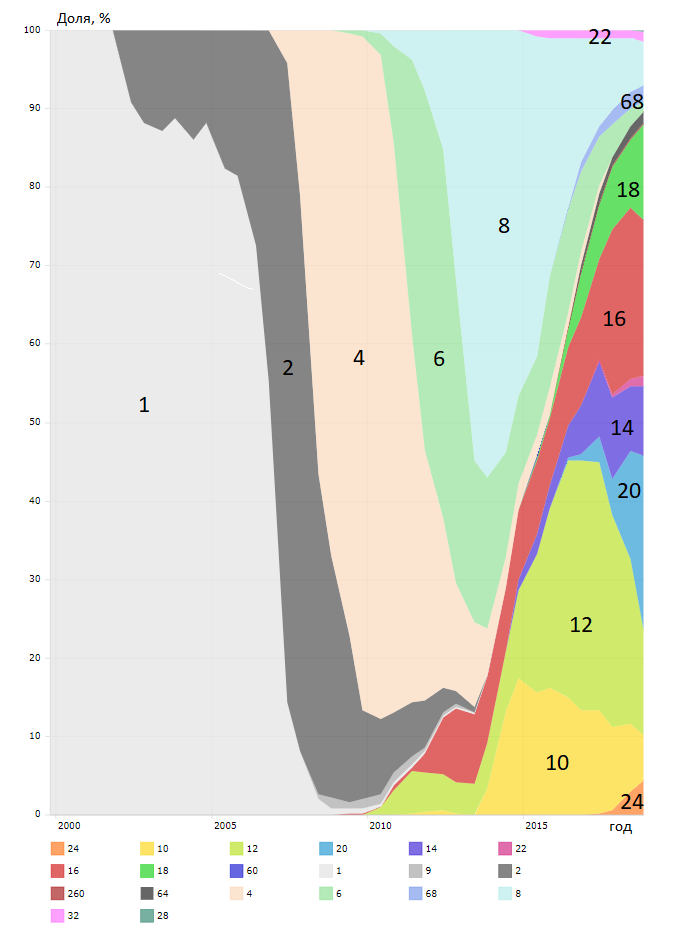
\includegraphics[width=1\linewidth]{graphPartOfMultiCoreProcessorFromYear}
		\caption{\textit{Частотность использования процессоров с различным числом ядер при создании суперкомпьютеров}}
		\label{graphPartOfMultiCoreProcessorFromYear:image}
	\end{figure}
	\parКак видим, активное использование двухъядерных процессоров в суперкомпьютерах началось уже в 2002 году, а примерно к 2005 году совершенно сошло на нет, тогда как в настольных компьютерах их применение в 2005 году лишь начиналось. На основании этого можно сделать простой прогноз распространённости многоядерных "настольных" процессоров к нужному году, если считать, что они в общих чертах повторяют развитие многоядерных архитектур суперкомпьютеров.
	\par
}